% ============================================================================
% Climate Meets the Economy: The DICE/CDICE Model, Solved with DEQNs
% Duration: ~70 minutes
% ============================================================================

\documentclass[aspectratio=169,11pt]{beamer}

% ---------- Theme and colors ----------
\usecolortheme{dove}
\setbeamertemplate{navigation symbols}{}
\setbeamertemplate{footline}{%
  \hfill\usebeamerfont{page number in head/foot}%
  \usebeamercolor[fg]{normal text}%
  \insertframenumber\,/\,\inserttotalframenumber\kern1em\vskip4pt}
\setbeamerfont{frametitle}{size=\huge}

% ---------- Packages ----------
\usepackage[utf8]{inputenc}
\usepackage[T1]{fontenc}
\usepackage{amsmath,amssymb,amsfonts}
\usepackage{bm}
\usepackage{graphicx}
\usepackage{tikz}
\usetikzlibrary{shapes,arrows.meta,positioning,calc,fit,backgrounds,patterns,decorations.pathreplacing}
\usepackage{pgfplots}
\pgfplotsset{compat=1.18}
\usepackage{booktabs}
\usepackage{hyperref}
\usepackage{multicol}
\usepackage{xcolor}
\usepackage{algorithm}
\usepackage{algorithmic}

% ---------- Custom colors ----------
\definecolor{uzhblue}{rgb}{0,0,0.5}
\definecolor{uzhgreylight}{RGB}{236,238,241}
\definecolor{uzhgreydark}{RGB}{81,86,94}
\definecolor{harvardcrimson}{RGB}{153,0,0}
\definecolor{unil@blue}{RGB}{0,140,204}
\definecolor{unil@black}{RGB}{35,31,32}
\definecolor{darkgreen}{RGB}{0,100,0}
\definecolor{darkred}{RGB}{139,0,0}
\definecolor{softblue}{RGB}{70,130,180}
\definecolor{softorange}{RGB}{230,159,0}
\definecolor{softgreen}{RGB}{0,158,115}

% ---------- Set beamer colors ----------
\setbeamercolor{frametitle}{bg=uzhgreylight, fg=uzhblue}
\setbeamercolor{title}{fg=uzhblue}
\setbeamercolor{structure}{fg=uzhblue}
\setbeamercolor{block title}{bg=unil@blue, fg=white}
\setbeamercolor{block body}{bg=uzhgreylight}
\setbeamercolor{block title alerted}{bg=darkred,fg=white}
\setbeamercolor{block body alerted}{bg=red!5}
\setbeamercolor{block title example}{bg=darkgreen,fg=white}
\setbeamercolor{block body example}{bg=green!5}
\setbeamercolor{item}{fg=unil@black}
\setbeamercolor{normal text}{fg=unil@black}

% ---------- Emphasis and hyperlinks ----------
\newcommand{\emphc}[1]{\textcolor{harvardcrimson}{#1}}
\hypersetup{colorlinks,linkcolor=harvardcrimson,urlcolor=harvardcrimson}

% ---------- Math commands ----------
\newcommand{\x}{\bm{x}}
\newcommand{\w}{\bm{w}}
\newcommand{\bb}{\bm{b}}
\newcommand{\z}{\bm{z}}
\newcommand{\W}{\bm{W}}
\newcommand{\X}{\bm{X}}
\renewcommand{\a}{\bm{a}}
\newcommand{\R}{\mathbb{R}}
\newcommand{\E}[1]{\mathbb{E}\!\left[#1\right]}
\newcommand{\nn}{\mathcal{N}_{\bm{\varphi}}}
\DeclareMathOperator*{\argmin}{arg\,min}
\DeclareMathOperator*{\argmax}{arg\,max}

% ---------- Title ----------
\title[CEMRACS 2026 $\cdot$ DICE]
{Computational and AI Methods in Climate Economics}
\subtitle{Lecture 2 (Part 2) --- Climate meets the economy: the DICE/CDICE model, solved with Deep Equilibrium Nets}
\author{Simon Scheidegger}
\institute[HEC Lausanne]{HEC Lausanne $\cdot$ Grantham Research Institute, LSE}
\date{July 15, 2026 \,$\cdot$\, CIRM, Marseille, France}

\begin{document}


% ============================================================================
% PART 0: TITLE & OUTLINE
% ============================================================================

% --- Slide 1: Title ---
{\setbeamercolor{background canvas}{bg=uzhgreylight}
\begin{frame}
\titlepage
\vspace{-0.4cm}
\begin{center}
{\footnotesize Based on: Folini, Friedl, K\"ubler \& Scheidegger (2025), ``The Climate in Climate Economics,''\\
\emph{Review of Economic Studies} 92(1), 299--338, and its Online Appendix.}\\[4pt]
{\footnotesize Production code: \url{https://github.com/ClimateChangeEcon/Climate_in_Climate_Economics}}\\[2pt]
{\footnotesize Materials: \url{https://github.com/sischei/cemracs2026_DEQN}}
\end{center}
\end{frame}
}

% --- Slide 2: Roadmap ---
\begin{frame}{Roadmap of This Lecture}
\vspace{0.2em}
\begin{columns}[T]
\column{0.48\textwidth}
\textbf{Part A}
\begin{itemize}
    \item \textbf{Part I.} Motivation: why climate economics, why IAMs, why this is computationally hard
    \item \textbf{Part II.} The DICE/CDICE model: economy, carbon cycle, temperature, damages, planner problem, social cost of carbon
\end{itemize}

\column{0.48\textwidth}
\textbf{Part B}
\begin{itemize}
    \item \textbf{Part III.} Solving DICE with DEQNs: time as a state, detrending, shadow prices as network outputs, the 8-component loss, training, accuracy
    \item \textbf{Part IV.} What is different compared to the Lecture 1 models (Brock--Mirman, IRBC)?
\end{itemize}
\end{columns}
\end{frame}

% --- Learning objectives ---
\begin{frame}{Learning objectives}
\textbf{By the end of this lecture you should be able to:}
\begin{itemize}
  \item Describe the building blocks of DICE/CDICE: neoclassical growth economy, 3-reservoir carbon cycle, 2-layer temperature dynamics, damages, and abatement
  \item Explain why an IAM is \emphc{non-stationary} and what that implies for recursive solution methods
  \item Map a non-stationary model onto DEQNs: time as a state variable, the Traeger time transformation, detrending to efficiency units
  \item Derive the 8-component DEQN loss from the planner's Lagrangian, including the Fischer--Burmeister treatment of $0 \leq \mu_t \leq 1$
  \item Read the social cost of carbon directly off the learned shadow prices, and contrast the whole recipe with the Lecture 1 models
\end{itemize}
\end{frame}


% ============================================================================
% PART I: MOTIVATION --- WHY CLIMATE ECONOMICS?
% ============================================================================

% --- Slide 4: Section Divider ---
\begin{frame}{}
\vfill
\begin{center}
{\Huge \textcolor{uzhblue}{\textbf{Part I}}}\\[12pt]
{\LARGE Why Climate Economics?}
\end{center}
\vfill
\end{frame}

% --- Slide 5: Climate change as economic threat ---
\begin{frame}{Climate Change as an Economic Threat}
\begin{columns}[T]
\column{0.48\textwidth}
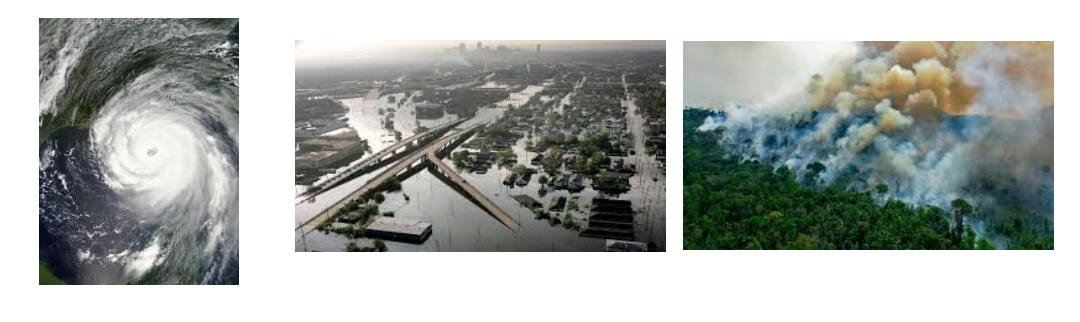
\includegraphics[width=\linewidth]{fig/global-warming.png}
{\footnotesize Observed global warming motivates the IAM feedback loop below.}

\column{0.50\textwidth}
\begin{itemize}
    \item Global warming is a growing threat to economic well-being.
    \item Tipping points place us in catastrophic danger.
    \item Impacts current and future generations in different regions very differently.
    \item Recent overviews: Dietz (2024), van der Ploeg and Rezai (2026), Fernandez-Villaverde, Gillingham, Scheidegger (2025).
\end{itemize}
\end{columns}
\end{frame}

% --- Slide 6: Why IAMs ---
\begin{frame}{Why Integrated Assessment Models (IAMs)?}
\begin{block}{IAM logic}
Couple the \emphc{economy} (output, investment, abatement, welfare) with the \emphc{climate system}
(carbon concentrations, temperature, damages).
\end{block}

\vspace{0.05cm}
\begin{center}
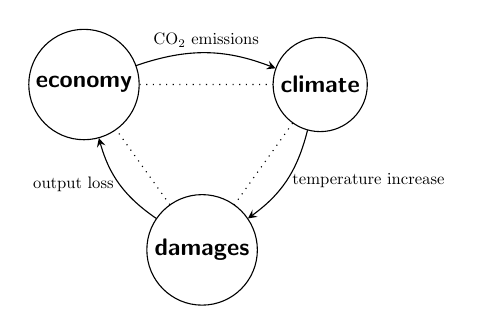
\begin{tikzpicture}[>=stealth, node distance=2cm, scale=0.60, transform shape]
    \tikzstyle{main node} = [circle, draw, minimum size=1.2cm, font=\sffamily\Large\bfseries]
    \node[main node] (economy) at (0,0) {economy};
    \node[main node] (climate) at (5,0) {climate};
    \node[main node] (damages) at (2.5,-3.5) {damages};
    \draw[->] (economy) to[bend left=20] node[above] {CO$_2$ emissions} (climate);
    \draw[->] (climate) to[bend left=20] node[right] {temperature increase} (damages);
    \draw[->] (damages) to[bend left=20] node[left] {output loss} (economy);
    \draw[dotted] (economy) -- (climate) -- (damages) -- (economy);
\end{tikzpicture}
\end{center}

\textbf{Output of interest:} social cost of carbon (SCC), optimal tax paths, welfare decomposition.
\vspace{-0.05cm}
\end{frame}

% --- Slide 7: Social cost of carbon ---
\begin{frame}{The Social Cost of Carbon (SCC)}
\begin{block}{Definition}
SCC at time $t$: marginal welfare cost of one extra unit of emissions, converted to consumption units.
\end{block}

\vspace{0.2cm}
\[
\mathrm{SCC}_t = -\frac{\partial V_t / \partial E_t}{\partial V_t / \partial C_t}
\]

\begin{columns}[T]
\column{0.49\textwidth}
\textbf{High SCC when}
\begin{itemize}
    \item Damages are steep
    \item Climate response is strong
    \item Discounting is low
    \item Tipping risk is material
\end{itemize}

\column{0.49\textwidth}
\textbf{Policy interpretation}
\begin{itemize}
    \item Tax path for carbon pricing
    \item Benchmark for regulation / cap-and-trade
    \item Input to cost-benefit analysis
    \item Why uncertainty matters: SCC is a \emphc{distribution}
\end{itemize}
\end{columns}
\end{frame}

% --- Slide 8: Why computationally hard ---
\begin{frame}{Why This Is Computationally Hard}
\begin{columns}[T]
\column{0.55\textwidth}
\begin{itemize}
    \item \textbf{Nonstationarity}: TFP, population, emissions intensity, and forcing paths all change exogenously over time.
    \item \textbf{Coupled dynamics}: economy and climate interact in both directions.
    \item \textbf{Long horizon}: welfare effects unfold over 100--300 years.
    \item \textbf{Curse of dimensionality}: nonlinearities, tipping hazards, constraints.
\end{itemize}

\column{0.42\textwidth}
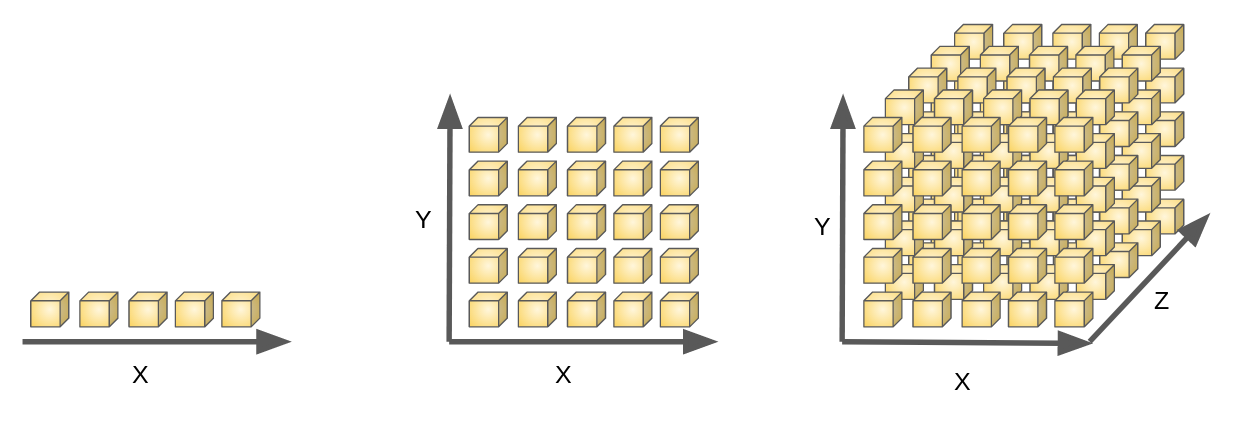
\includegraphics[width=0.84\linewidth]{fig/cod.png}\\[4pt]
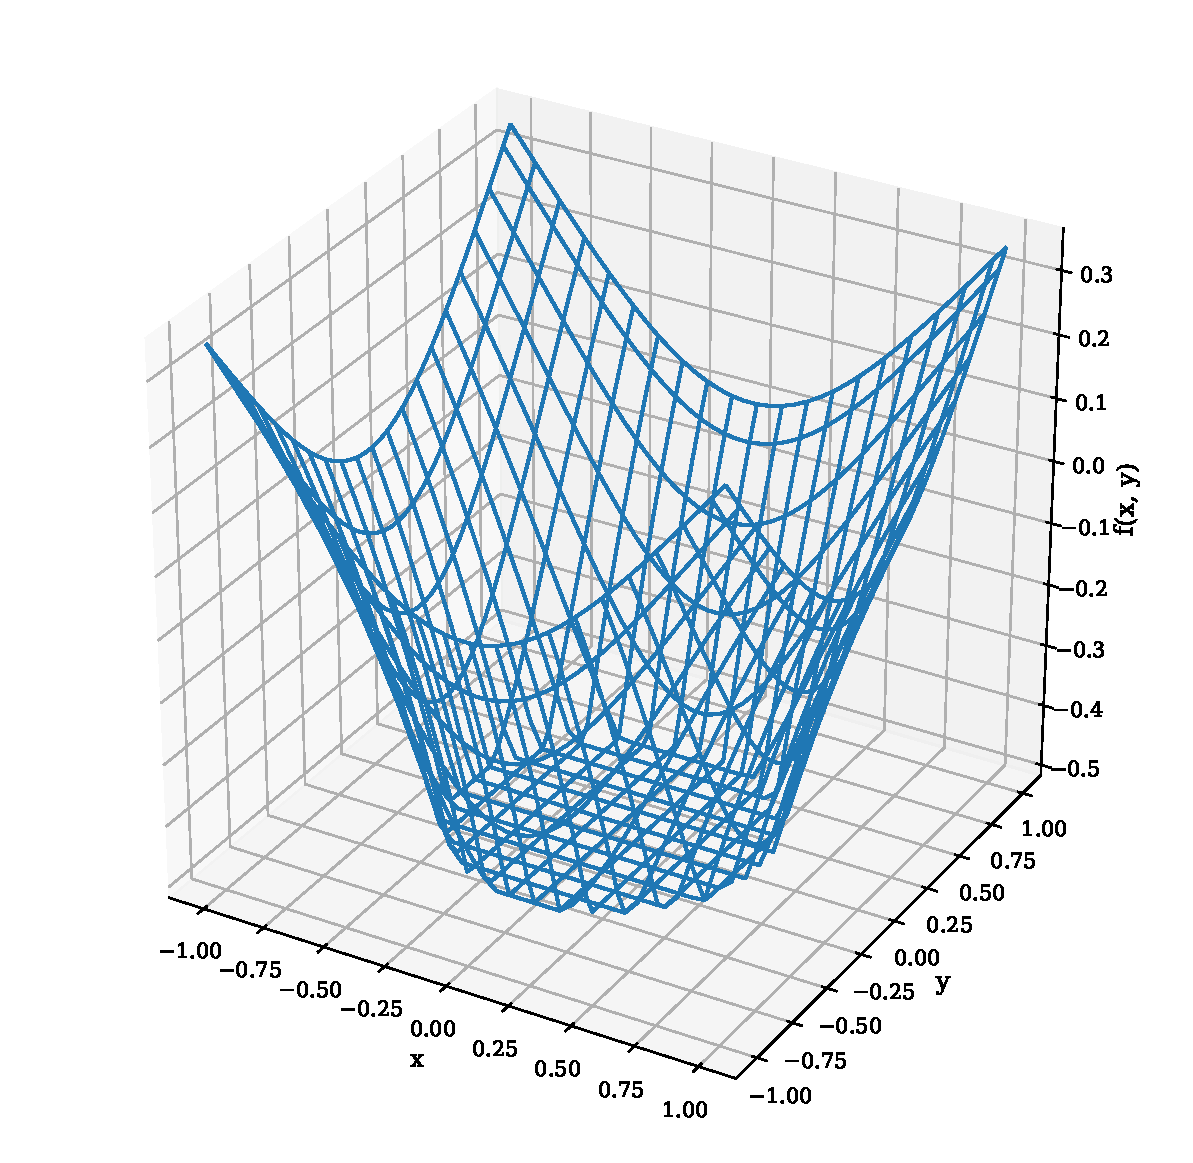
\includegraphics[width=0.84\linewidth]{fig/examplefunc.pdf}
\end{columns}
\end{frame}

% --- Slide 9: This lecture's approach ---
\begin{frame}{This Lecture's Approach}
\begin{itemize}
    \item \textcolor{blue}{\textbf{Take the DEQN machinery from Lecture 1}} --- policy networks trained on the residuals of equilibrium conditions along simulated paths --- and apply it to a \emphc{non-stationary} climate--economy model.
    \item \textcolor{blue}{\textbf{Solve the deterministic CDICE benchmark globally}}, so that the social cost of carbon comes out as a by-product of the learned shadow prices.
\end{itemize}

\vspace{0.2cm}
\begin{enumerate}
    \item State the \textbf{DICE/CDICE model}: economy $+$ carbon cycle $+$ temperature $+$ damages.
    \item Map it onto \textbf{deep equilibrium nets}: time as a state, detrending, multipliers as outputs.
    \item Train on the \textbf{8 first-order conditions} and validate with error statistics.
\end{enumerate}

\vspace{0.2cm}
{\footnotesize \emphc{Connection to Part 1 of this lecture:} once the model can be solved fast and reliably, GP surrogates and Bayesian active learning turn the SCC into a \emph{distribution} over uncertain parameters.}
\end{frame}


% ============================================================================
% PART II: THE DICE/CDICE MODEL
% ============================================================================

% --- Slide 10: Section Divider ---
\begin{frame}{}
\vfill
\begin{center}
{\Huge \textcolor{uzhblue}{\textbf{Part II}}}\\[12pt]
{\LARGE The DICE/CDICE Model}
\end{center}
\vfill
\end{frame}

% --- Slide 11: DICE baseline ---
\begin{frame}{DICE: A Minimal Global IAM}
\small
\begin{columns}[T]
\column{0.56\textwidth}
\textbf{State variables}
\begin{itemize}
    \item Economic stock: $K_t$
    \item Carbon stocks: $M_t^{\mathrm{AT}}, M_t^{\mathrm{UO}}, M_t^{\mathrm{LO}}$
    \item Temperature states: $T_t^{\mathrm{AT}}, T_t^{\mathrm{OC}}$
    \item Exogenous trends: population $L_t$, TFP $A_t$, carbon intensity $\sigma_t$
\end{itemize}

\textbf{Controls}
\begin{itemize}
    \item Consumption $C_t$ (equivalently investment $I_t$)
    \item Abatement rate $\mu_t \in [0,1]$
\end{itemize}

\column{0.41\textwidth}
\begin{exampleblock}{Why DICE is influential}
\begin{itemize}
    \item Transparent
    \item Fast to evaluate
    \item Policy-facing
    \item Benchmark for extensions
\end{itemize}
\end{exampleblock}
\end{columns}

\begin{alertblock}{Challenge}
Fast is useful, but only if the climate module is calibrated consistently with climate science --- this is where \emphc{CDICE} comes in.
\end{alertblock}
\end{frame}

% --- Slide 12: Model anatomy ---
\begin{frame}{Anatomy: One Economy, Two Physical Blocks}
\begin{center}
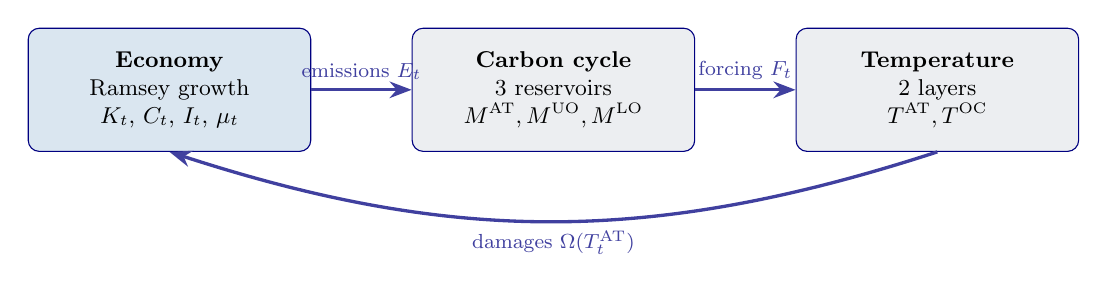
\begin{tikzpicture}[scale=0.92, transform shape,
    blk/.style={rectangle, draw=uzhblue, fill=uzhgreylight, rounded corners=4pt,
                minimum width=3.9cm, minimum height=1.7cm, align=center, font=\small},
    arr/.style={-{Stealth[length=2.8mm]}, very thick, uzhblue!75}
]
\node[blk, fill=softblue!20] (econ) at (0,0)
      {\textbf{Economy}\\Ramsey growth\\$K_t$, $C_t$, $I_t$, $\mu_t$};
\node[blk] (carbon) at (5.3,0)
      {\textbf{Carbon cycle}\\3 reservoirs\\$M^{\mathrm{AT}}, M^{\mathrm{UO}}, M^{\mathrm{LO}}$};
\node[blk] (temp) at (10.6,0)
      {\textbf{Temperature}\\2 layers\\$T^{\mathrm{AT}}, T^{\mathrm{OC}}$};
\draw[arr] (econ) -- node[above, font=\footnotesize] {emissions $E_t$} (carbon);
\draw[arr] (carbon) -- node[above, font=\footnotesize] {forcing $F_t$} (temp);
\draw[arr] (temp.south) to[bend left=18] node[below, font=\footnotesize] {damages $\Omega(T^{\mathrm{AT}}_t)$} (econ.south);
\end{tikzpicture}
\end{center}

\vspace{0.3cm}
\begin{itemize}
    \item The carbon cycle affects temperature, \emphc{but not vice versa}: the physical part is a one-directional chain, closed only through the damage function.
    \item All coefficients carry an explicit time step $\Delta_t$: DICE-2007 uses $\Delta_t = 10$ years, DICE-2016 uses $5$, CDICE uses $\Delta_t = 1$ --- one \emphc{generic formulation} covers all of them.
\end{itemize}
\end{frame}

% --- Slide 13: Economy: production and capital ---
\begin{frame}{The Economy I: Production and Capital}
Standard neoclassical growth, with output produced from capital and effective labor:
\begin{align*}
    Y^{\text{Gross}}_t &= (A_t L_t)^{1-\alpha}\, K_t^{\alpha}, \\
    K_{t+1} &= (1-\delta^K)^{\Delta_t} K_t + \Delta_t I_t .
\end{align*}

\vspace{0.2cm}
\begin{columns}[T]
\column{0.48\textwidth}
\textbf{Ingredients}
\begin{itemize}
    \item $A_t$: total factor productivity (exogenous trend)
    \item $L_t$: population $=$ labor (exogenous trend)
    \item $\alpha = 0.3$, $\delta^K = 0.1$ per year
\end{itemize}

\column{0.48\textwidth}
\begin{block}{So far, so familiar}
Without the climate block this is the deterministic growth model from Lecture 1 --- \emphc{except} that $A_t$ and $L_t$ follow exogenous time paths, so the model has no steady state to converge to.
\end{block}
\end{columns}
\end{frame}

% --- Slide 14: Economy: damages and abatement ---
\begin{frame}{The Economy II: Damages and Abatement}
\small
Warming destroys a fraction of gross output; abating emissions costs another fraction:
\vspace{-0.1cm}
\begin{align*}
    \Omega_t &= \psi_1 T^{\text{AT}}_{t} + \psi_2 \left(T^{\text{AT}}_{t}\right)^2 \ \text{(damages)},
    \qquad \Theta_{t} = \theta_{1,t}\, \mu_t^{\theta_2} \ \text{(abatement cost)}, \\
    Y_t &= Y^{\text{Gross}}_t \left(1 - \Theta_t - \Omega_t \right),
    \qquad C_t = Y_t - I_t.
\end{align*}

\vspace{-0.1cm}
\begin{columns}[T]
\column{0.36\textwidth}
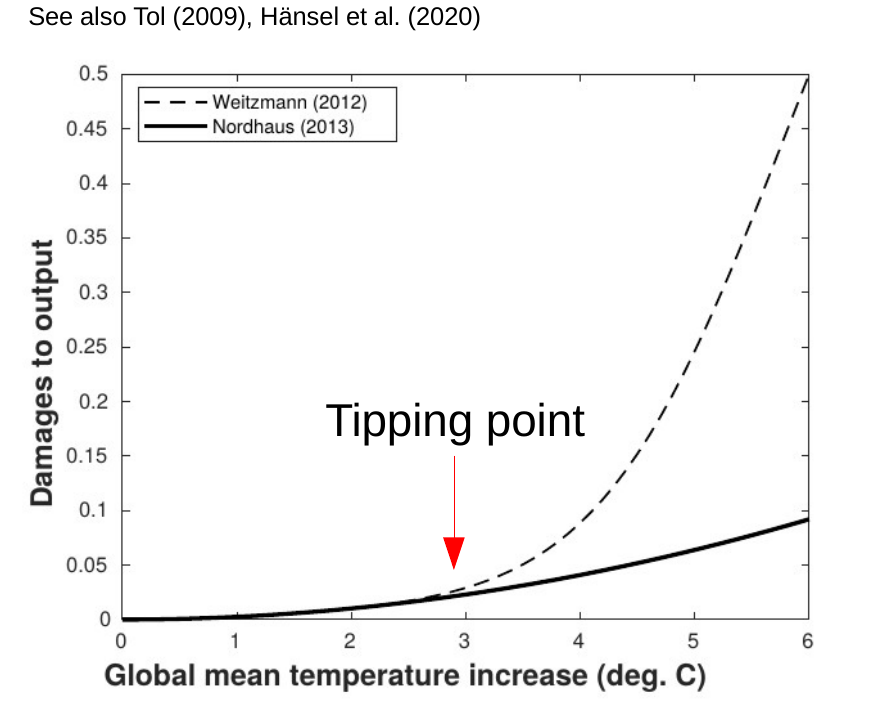
\includegraphics[width=0.88\linewidth]{fig/damage.png}
{\scriptsize Damage fraction $\Omega(T)$: share of gross output lost at warming $T$.}

\column{0.60\textwidth}
\begin{itemize}\itemsep2pt
    \item DICE-2016: $\psi_1 = 0$, $\psi_2 = 0.00236$; abatement exponent $\theta_2 = 2.6$; $\theta_{1,t}$ tracks a falling backstop price.
    \item $\mu_t \in [0,1]$: fraction of industrial emissions abated; $\mu_t = 1$ means the \emphc{backstop technology} eliminates all emissions.
    \item The degree of convexity of $\Omega$ is key for optimal taxes (Weitzman 2012); tipping variants are much steeper.
    \item DICE-2007 uses the hyperbolic form $\Omega_t = 1/(1 + \psi_1 T^{\text{AT}}_t + \psi_2 (T^{\text{AT}}_t)^2)$.
\end{itemize}
\end{columns}
\end{frame}

% --- Slide 15: Preferences ---
\begin{frame}{The Economy III: Preferences}
A social planner maximizes population-weighted CRRA utility of per-capita consumption:
\[
U = \sum_{t=0}^{T} \beta^{t}\, \Delta_t\,
\frac{\left(\frac{C_t}{L_t}\right)^{1-1/\psi} - 1}{1-1/\psi}\, L_t ,
\qquad
\beta = \frac{1}{(1+\rho)^{\Delta_t}} .
\]

\vspace{0.3cm}
\begin{columns}[T]
\column{0.48\textwidth}
\textbf{Parameters (DICE-2016/CDICE)}
\begin{itemize}
    \item IES $\psi = 0.69$
    \item Rate of time preference $\rho = 0.015$ per year
    \item Initial capital $K_0 = 223$ trillion USD (2015)
\end{itemize}

\column{0.48\textwidth}
\begin{block}{Discounting is the battleground}
With effects unfolding over centuries, $\rho$ and $\psi$ dominate the size of the SCC --- one reason global sensitivity analysis (Part 1 of this lecture) matters so much in climate economics.
\end{block}
\end{columns}
\end{frame}

% --- Slide 16: Carbon cycle ---
\begin{frame}{The Climate I: Carbon Cycle (3-Box Model)}
\small
Three carbon reservoirs --- atmosphere (AT), upper ocean (UO), lower ocean (LO) --- exchange carbon as a \emphc{linear dynamical system}, $M_{t+1} = (I + \Delta_t B)\, M_t + \Delta_t E_t$:
\begin{align*}
M^{\text{AT}}_{t+1} &= (1- \Delta_t b_{12}) M^{\text{AT}}_{t} + \Delta_t b_{12} \tfrac{M^{\text{AT}}_{\text{EQ}}}{M^{\text{UO}}_{\text{EQ}}} M^{\text{UO}}_{t} +  \Delta_t E_t ,\\
M^{\text{UO}}_{t+1} &= \Delta_t b_{12} M^{\text{AT}}_{t} + (1- \Delta_t b_{12} \tfrac{M^{\text{AT}}_{\text{EQ}}}{M^{\text{UO}}_{\text{EQ}}} - \Delta_t b_{23}) M^{\text{UO}}_{t} + \Delta_t b_{23} \tfrac{M^{\text{UO}}_{\text{EQ}}}{M^{\text{LO}}_{\text{EQ}}} M^{\text{LO}}_{t} ,\\
M^{\text{LO}}_{t+1} &= \Delta_t b_{23} M^{\text{UO}}_{t} + (1-\Delta_t b_{23} \tfrac{M^{\text{UO}}_{\text{EQ}}}{M^{\text{LO}}_{\text{EQ}}}) M^{\text{LO}}_{t} .
\end{align*}

Emissions couple the economy into the carbon cycle:
\[
\boxed{\;E_t = \sigma_t\, Y^{\text{Gross}}_{t}\, (1-\mu_t) + E^{\text{Land}}_t\;}
\]

\begin{itemize}
    \item Mass conservation: columns of $B$ sum to zero; no direct AT $\leftrightarrow$ LO exchange.
    \item Free parameters: transfer rates $b_{12}$, $b_{23}$ and equilibrium ratios $M^{\text{AT}}_{\text{EQ}}/M^{\text{UO}}_{\text{EQ}}$, $M^{\text{UO}}_{\text{EQ}}/M^{\text{LO}}_{\text{EQ}}$.
\end{itemize}
\end{frame}

% --- Slide 17: Temperature ---
\begin{frame}{The Climate II: Temperature (2-Layer Energy Balance)}
\small
Atmosphere-plus-upper-ocean layer $T^{\text{AT}}$ and deep-ocean layer $T^{\text{OC}}$:
\begin{align*}
T^{\text{AT}}_{t+1} &= T^{\text{AT}}_{t} + \Delta_t c_1 F_t  - \Delta_t c_1 \frac{F_{\text{2XCO2}}}{T_{\text{2XCO2}}} T^{\text{AT}}_{t} - \Delta_t c_1 c_3 \left(T^{\text{AT}}_{t}-T^{\text{OC}}_{t}\right),    \\
T^{\text{OC}}_{t+1} &= T^{\text{OC}}_{t} + \Delta_t c_4 \left(T^{\text{AT}}_{t}  - T^{\text{OC}}_{t}\right),
\end{align*}
driven by radiative forcing from atmospheric carbon (plus exogenous non-CO$_2$ forcing):
\[
F_{t} = F_{\text{2XCO2}} \frac{\log\!\left(M^{\text{AT}}_{t}/M^{\text{AT}}_{\text{base}}\right)}{\log(2)} + F^{EX}_{t}.
\]

\begin{alertblock}{Key parameter: equilibrium climate sensitivity (ECS)}
$T_{\text{2XCO2}}$ is the long-run warming from a doubling of atmospheric CO$_2$; the feedback strength is $\lambda = F_{\text{2XCO2}}/T_{\text{2XCO2}}$. Physically, $1/c_1$ and $c_3/c_4$ are heat capacities, $c_3$ the heat-exchange coefficient.
\end{alertblock}
\end{frame}

% --- Slide 18: Exogenous trends ---
\begin{frame}{Exogenous Trends: The Source of Non-Stationarity}
\footnotesize
Six deterministic, time-dependent processes drive the model (DICE-2016 forms, annual $t$):
\begin{align*}
&\text{Population:} & L_{t} &= L_{0} + \left(L_{\infty}-L_{0}\right)\left(1-e^{-\Delta_t\delta^{L}t}\right)
&&\text{growth } g^{L}_{t} \\
&\text{TFP:} & A_t &= A_0 \exp\!\left( \tfrac{\Delta_t g^A_0 (1 - e^{-\Delta_t\delta^A t})}{\Delta_t\delta^A} \right)
&&\text{growth } g^{A}_{t} = \Delta_t g^A_0 e^{-\Delta_t\delta^A t} \\
&\text{Carbon intensity:} & \sigma_{t} &= \sigma_{0}\exp\!\left( \tfrac{\Delta_t g^\sigma_0}{\log(1+ \Delta_t\delta^\sigma)}\left( (1 + \Delta_t\delta^\sigma)^t -1 \right) \right) \\
&\text{Backstop cost:} & \theta_{1,t} &= \frac{p^{\text{back}}_{0} e^{-g^{\text{back}}t}\, 1000 \cdot \text{c2co2} \cdot \sigma_{t}}{\theta_{2}} \\
&\text{Land emissions:} & E_{\text{Land},t} &= E_{\text{Land},0}\, e^{-\Delta_t\delta^{\text{Land}}t} \\
&\text{Non-CO$_2$ forcing:} & F^{EX}_{t} &= F^{EX}_{0} + \tfrac{1}{\text{T}/\Delta_t}(F^{EX}_{1} -F^{EX}_{0}) \min(t, \text{T}/\Delta_t)
\end{align*}

\begin{alertblock}{Why this matters for us}
Because $A_t, L_t, \sigma_t, \theta_{1,t}, E_{\text{Land},t}, F^{EX}_t$ all depend on calendar time, the optimal policy is \emphc{not time-invariant}: $C_t \neq C(K_t, M_t, T_t)$ alone. This single fact drives most of the DEQN design choices in Part III.
\end{alertblock}
\end{frame}

% --- Slide 19: Why recalibrate -> CDICE ---
\begin{frame}{From DICE to CDICE: Why Recalibrate?}
\small
\begin{itemize}
    \item Climate emulators must reproduce benchmark behavior from climate-science model archives (CMIP5).
    \item Earlier critiques highlighted major discrepancies for common IAM calibrations: DICE-2016's carbon cycle and temperature blocks are \emphc{not in balance} and overreact to changes in inputs.
    \item Folini et al.\ (2025) show the \emphc{functional form can remain simple}, but the parameters require systematic calibration --- the result is \emphc{CDICE}.
\end{itemize}

\vspace{0.1cm}
\begin{center}
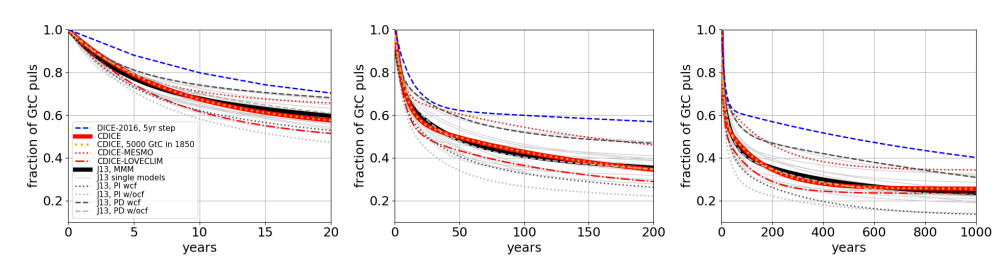
\includegraphics[width=0.60\textwidth]{fig/CDICE-vs-DICE.png}
\end{center}
\vspace{-0.1cm}
{\footnotesize CDICE recalibrates the reduced-form climate emulator to climate-science benchmarks, on an annual time step ($\Delta_t = 1$).}
\end{frame}

% --- Slide 20: Calibration tests ---
\begin{frame}{CDICE Calibration: Benchmarks from Climate Science}
\scriptsize
\begin{center}
\begin{tabular}{lll}
\toprule
\textbf{Test} & \textbf{Targets} & \textbf{Use} \\
\midrule
1. Carbon pulse (100 GtC) & Atmospheric retention path & Calibrate carbon cycle \\
2. 4$\times$CO$_2$ step & Temperature impulse response & Calibrate temperature block \\
3. 1\% CO$_2$/year & Transient climate response (TCR) & Out-of-sample validation \\
4. Historical + RCP & Realistic forcing paths & End-to-end validation \\
\bottomrule
\end{tabular}
\end{center}

\vspace{0.2cm}
\begin{columns}[T]
\column{0.48\textwidth}
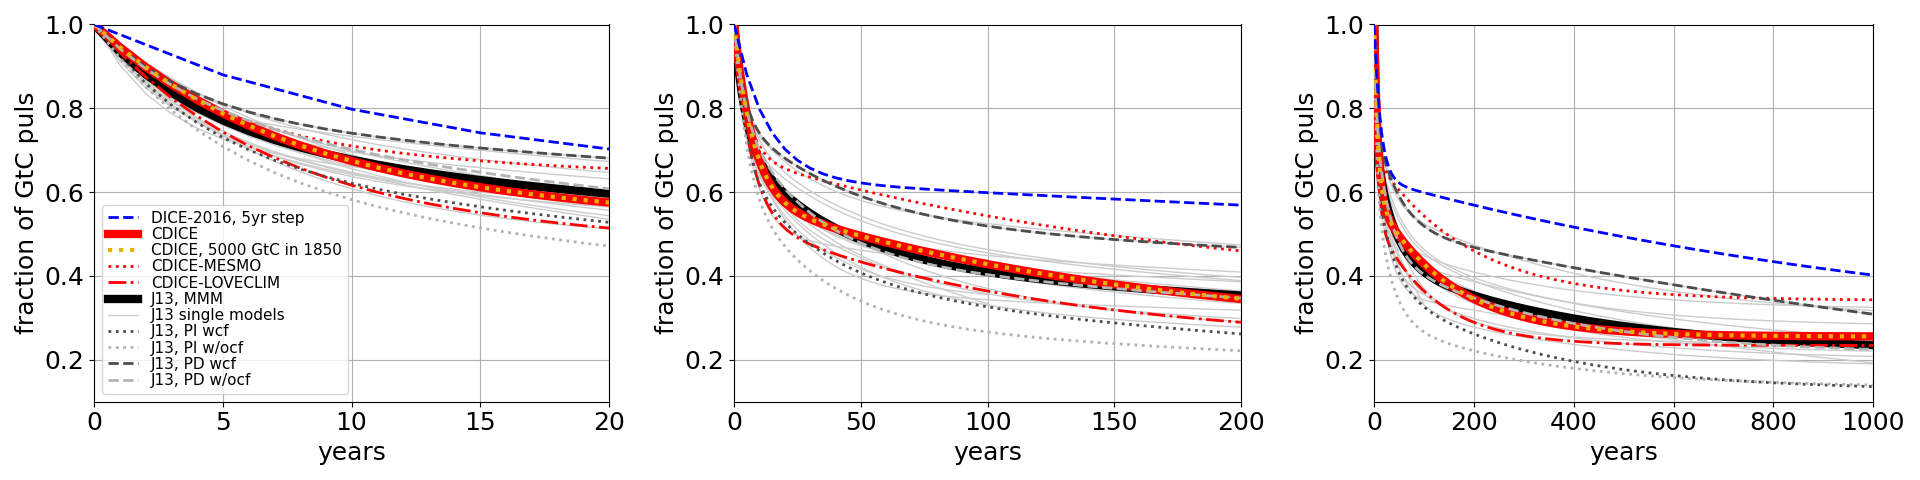
\includegraphics[width=\linewidth]{fig/CCBM_100GtC_Puls.png}
{\footnotesize Carbon-pulse response.}

\column{0.48\textwidth}
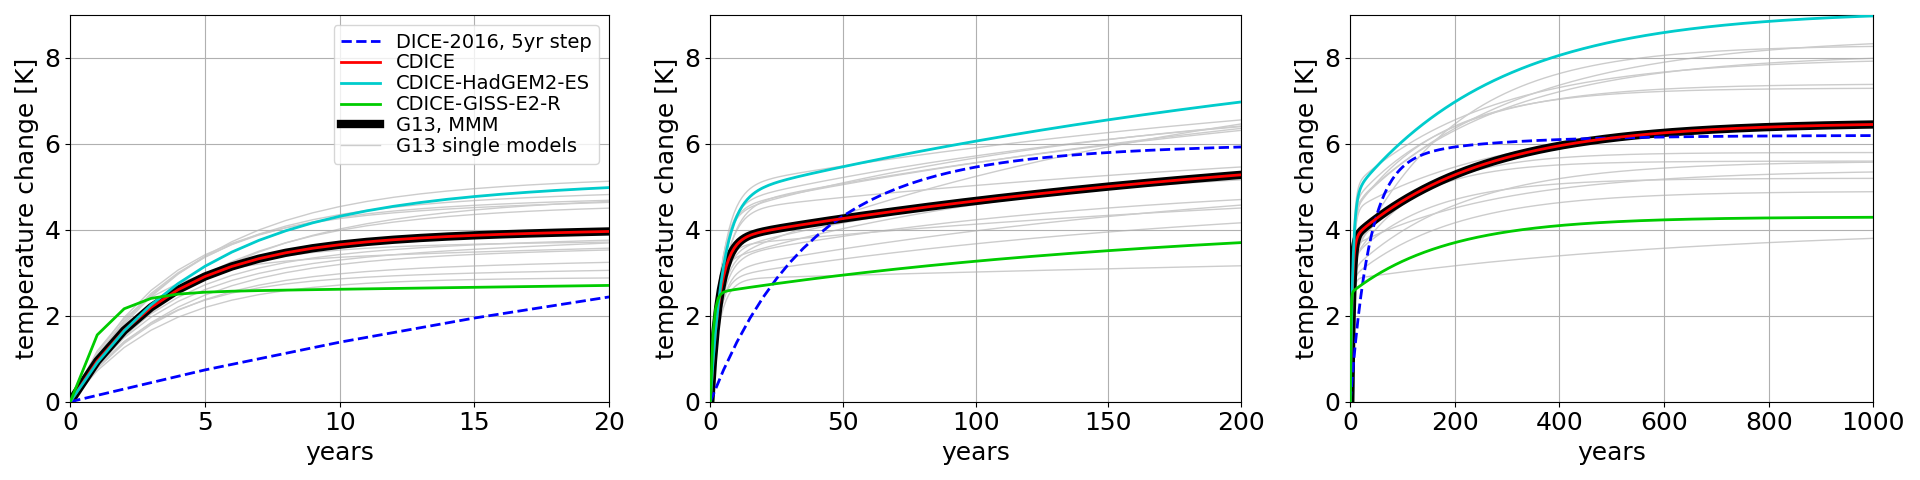
\includegraphics[width=\linewidth]{fig/TempBM_4xCO2_on_PI.png}
{\footnotesize Temperature response to a $4\times$CO$_2$ forcing step.}
\end{columns}
\end{frame}

% --- Slide 21: Calibration table ---
\begin{frame}{CDICE at a Glance: Key Parameter Values}
\scriptsize
\setlength{\tabcolsep}{3pt}
\begin{columns}[T]
\column{0.40\textwidth}
{\footnotesize\textbf{Economy (annual)}}
\begin{center}
\begin{tabular}{lcc}
\toprule
 & Symbol & CDICE \\
\midrule
Capital depreciation & $\delta^K$ & 0.1 \\
Capital share & $\alpha$ & 0.3 \\
Damage (quadratic) & $\psi_2$ & 0.00236 \\
Abatement exponent & $\theta_2$ & 2.6 \\
IES & $\psi$ & 0.69 \\
Time preference & $\rho$ & 0.015 \\
Initial capital [tn USD] & $K_0$ & 223 \\
\bottomrule
\end{tabular}
\end{center}

\column{0.57\textwidth}
{\footnotesize\textbf{Climate (annual)}}
\begin{center}
\begin{tabular}{lcc}
\toprule
 & Symbol & CDICE \\
\midrule
Carbon transfer AT$\to$UO & $b_{12}$ & 0.054 \\
Carbon transfer UO$\to$LO & $b_{23}$ & 0.0082 \\
Eq.\ masses AT/UO/LO [GtC] & $M_{\text{EQ}}$ & 607, 489, 1281 \\
Initial masses 2015 [GtC] & $M_{\text{INI}}$ & 851, 628, 1323 \\
Temp.\ coefficients & $c_1, c_3, c_4$ & 0.137, 0.73, 0.00689 \\
Forcing CO$_2$ doubling & $F_{\text{2XCO2}}$ & 3.45 W/m$^2$ \\
ECS & $T_{\text{2XCO2}}$ & 3.25\,\textdegree C \\
Initial temperatures & $T_0$ & 1.1, 0.27\,\textdegree C \\
\bottomrule
\end{tabular}
\end{center}
\end{columns}

\vspace{0.25cm}
{\footnotesize Full generic calibration tables (DICE-2007, DICE-2016, CDICE side by side): Online Appendix of Folini et al.\ (2025) --- in your \texttt{readings/} folder.}
\end{frame}

% --- Slide 22: Planner problem ---
\begin{frame}{The Planner's Problem (Annual CDICE, $\Delta_t = 1$)}
\vspace{-0.15cm}
\resizebox{\linewidth}{!}{%
\begin{minipage}{1.30\linewidth}
\begin{align*}
  & \max_{\left\{C_{t}, \mu_t\right\}_{t=0}^{\infty}} \sum_{t=0}^{\infty} \beta^t
  \frac{\left(\frac{C_t}{L_t}\right)^{1-1/\psi} -1}{1-1/\psi} L_t\\
  %
  \text{s.t.}\quad
  & K_{t+1} = \left(1 - \Omega\left(T_{\text{AT},t}\right) -\Theta\left(\mu_{t}\right)\right)
    K_t^{\alpha} \left(A_{t}L_t\right)^{1-\alpha} + (1-\delta) K_t - C_{t} && \left(\lambda_{t}\right)  \\
  & M^{\text{AT}}_{t+1} = \left(1 - b_{12}\right) M^{\text{AT}}_{t} + b_{12} \tfrac{M^{\text{AT}}_{\text{EQ}}}{M^{\text{UO}}_{\text{EQ}}} M^{\text{UO}}_{t} + \sigma_t (1-\mu_t) K_t^{\alpha} \left(A_{t}L_t\right)^{1-\alpha}  + E^{\text{Land}}_t && \left(\nu^{\text{AT}}_{t}\right)\\
  & M^{\text{UO}}_{t+1} = b_{12}M^{\text{AT}}_{t} + \left(1 - b_{12} \tfrac{M^{\text{AT}}_{\text{EQ}}}{M^{\text{UO}}_{\text{EQ}}} - b_{23}\right)M^{\text{UO}}_{t} + b_{23} \tfrac{M^{\text{UO}}_{\text{EQ}}}{M^{\text{LO}}_{\text{EQ}}}  M^{\text{LO}}_{t} && \left(\nu^{\text{UO}}_{t}\right)  \\
  & M^{\text{LO}}_{t+1} = b_{23}M^{\text{UO}}_{t} + \left(1 - b_{23} \tfrac{M^{\text{UO}}_{\text{EQ}}}{M^{\text{LO}}_{\text{EQ}}} \right)M^{\text{LO}}_{t} && \left(\nu^{\text{LO}}_{t}\right)\\
  & T^{\text{AT}}_{t+1} = T^{\text{AT}}_{t} + c_1 \left(F_{\text{2XCO2}} \tfrac{\log(M^{\text{AT}}_{t}/M^{\text{AT}}_{\text{base}})}{\log(2)} + F^{EX}_{t} \right)  - c_1 \tfrac{F_{\text{2XCO2}}}{T_{\text{2XCO2}}}T^{\text{AT}}_{t}- c_1c_3 \left(T^{\text{AT}}_{t}-T^{\text{OC}}_{t}\right) && \left(\eta^{\text{AT}}_{t}\right)\\
  & T^{\text{OC}}_{t+1} = T^{\text{OC}}_{t} + c_4 \left(T^{\text{AT}}_{t}  - T^{\text{OC}}_{t}\right) && \left(\eta^{\text{OC}}_{t}\right)\\
  & 0 \leq \mu_t \leq 1 && \left( \lambda^{\mu}_{t} \right)
\end{align*}
\end{minipage}
}

{\small One economic constraint, \emphc{five climate constraints}, one inequality constraint --- the Lagrange/KKT multipliers in parentheses will all reappear as \emphc{network outputs} in Part III.}
\end{frame}

% --- Slide 23: SCC and carbon tax ---
\begin{frame}{The SCC and the Optimal Carbon Tax in DICE}
The SCC is the planner's marginal rate of substitution between atmospheric carbon and capital:
\[
\boxed{\;\mathrm{SCC}_t = -\frac{\partial V_t / \partial M_{\text{AT},t}}{\partial V_t / \partial K_t}\;}
\]

In the optimum, an interior abatement policy $0 < \mu_t < 1$ equates the SCC with the marginal abatement cost, which defines the optimal carbon tax:
\[
\mathrm{CT}_t = \frac{\theta_{1,t}\, \theta_2\, \mu_t^{\theta_2-1}}{\sigma_t}.
\]

\vspace{0.3cm}
\begin{block}{Preview of Part III}
$\partial V_t / \partial M_{\text{AT},t}$ and $\partial V_t / \partial K_t$ are exactly the \emphc{shadow prices} $\nu^{\text{AT}}_t$ and $\lambda_t$ of the planner problem. The DEQN learns both as network outputs --- so the SCC comes \emphc{for free} with the solution, no numerical differentiation of a value function required.
\end{block}
\end{frame}


% ============================================================================
% PART III: SOLVING DICE WITH DEQNs
% ============================================================================

% --- Slide 24: Section Divider ---
\begin{frame}{}
\vfill
\begin{center}
{\Huge \textcolor{uzhblue}{\textbf{Part III}}}\\[12pt]
{\LARGE Solving DICE with Deep Equilibrium Nets}
\end{center}
\vfill
\end{frame}

% --- Slide 25: DEQN recap ---
\begin{frame}{DEQN in a Nutshell (Recap from Lecture 1)}
\small
Approximate the unknown policy $p: X \to Y \subset \R^K$ of a model characterized by first-order equilibrium conditions $\mathbf{G}(\x, p(\x)) = \bm{0}$ for all $\x \in X$ with a neural network $p(\x) \approx \nn(\x)$, and use the residual of those conditions as the loss:
\[
\ell_{\bm{\varphi}} := \frac{1}{N_{\text{path length}}}\sum_{\x_t \,\text{on sim.\ path}}\ \sum_{m=1}^{N_{eq}}\left(G_{m}(\x_t, \nn(\x_t))\right)^2 ,
\qquad
\varphi^{\prime}_{k}=\varphi_{k} - \alpha^{\text{learn}} \frac{\partial \ell(\bm{\varphi})}{\partial \varphi_{k}} .
\]

\vspace{0.15cm}
\textbf{Four building blocks:}
\begin{enumerate}
    \item A deep neural network approximating the equilibrium policies (Xavier/Glorot init);
    \item A loss function: the error in the equilibrium conditions;
    \item An updating mechanism: gradient descent (Adam);
    \item A sampling method: states visited by \emphc{simulating the model} under the current policy.
\end{enumerate}

\vspace{0.1cm}
{\footnotesize Notation: we write $\bm{\varphi}$ for the network weights (Lecture 1 used $\rho$, which here denotes the rate of time preference).}
\end{frame}

% --- Slide 26: What breaks ---
\begin{frame}{What Breaks When We Point This at DICE?}
\footnotesize
In Lecture 1, every model (Brock--Mirman, stochastic growth, IRBC) was \emphc{stationary}: a time-invariant policy on an ergodic state space. DICE is not.

\vspace{0.2em}
\begin{columns}[T]
\column{0.48\textwidth}
\begin{alertblock}{Three obstacles}
\begin{enumerate}
    \item \textbf{Non-stationarity}: exogenous trends make the policy depend on calendar time.
    \item \textbf{Unbounded inputs and levels}: $t \in [0,\infty)$; $K_t, C_t$ grow without bound along the trend.
    \item \textbf{Occasionally binding constraint}: $\mu_t \leq 1$ once the backstop becomes cheap.
\end{enumerate}
\end{alertblock}

\column{0.48\textwidth}
\begin{exampleblock}{Three fixes}
\begin{enumerate}
    \item Add \textbf{time as an exogenous state}.
    \item Compress time (\textbf{Traeger transform}) and \textbf{detrend} to efficiency units.
    \item Smooth KKT via \textbf{Fischer--Burmeister} --- the same trick as IRBC irreversibility.
\end{enumerate}
\end{exampleblock}
\end{columns}

\vspace{0.3em}
And one genuinely new feature: the network must also output \emphc{shadow prices of the climate states}.
\end{frame}

% --- Slide 27: Time as a state ---
\begin{frame}{Fix 1: Time as an Exogenous State Variable}
The state of the economy at time $t$:
\[
\x_t := \left(k_t,\, M^{\text{AT}}_{t},\, M^{\text{UO}}_{t},\, M^{\text{LO}}_{t},\, T^{\text{AT}}_{t},\, T^{\text{OC}}_{t},\, t \right)^T \in \R^7 .
\]

\begin{itemize}
    \item Six \emphc{endogenous} states: detrended capital $k_t$, three carbon masses, two temperatures.
    \item One \emphc{exogenous} state: physical time $t$, which indexes all the deterministic trends $A_t, L_t, \sigma_t, \theta_{1,t}, E_{\text{Land},t}, F^{EX}_t$.
\end{itemize}

\vspace{0.3cm}
\begin{block}{Interpretation}
Feeding $t$ to the network restores a \emphc{recursive} formulation: the policy is again a time-invariant function --- of an enlarged state that includes the calendar. Dimensionality here comes from the \emphc{climate block}, not from many countries as in the IRBC.
\end{block}
\end{frame}

% --- Slide 28: Traeger transform ---
\begin{frame}{Fix 2a: Compressing the Infinite Horizon (Traeger 2014)}
\small
Physical time is unbounded, $t \in [0, \infty)$ --- a poor input for a neural network. Map it into the unit interval via the strictly monotonic transformation
\[
\boxed{\;\tau = 1 - \exp\left(-\vartheta t\right), \qquad \tau \in (0, 1]\;}
\qquad\text{with inverse}\qquad
t = -\frac{\ln\left(1-\tau\right)}{\vartheta}.
\]

\begin{columns}[T]
\column{0.48\textwidth}
\begin{center}
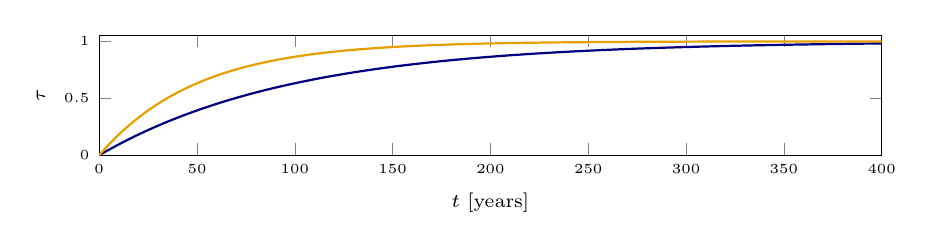
\begin{tikzpicture}
\begin{axis}[width=0.95\linewidth, height=3.1cm,
    xlabel={$t$ [years]}, ylabel={$\tau$},
    xmin=0, xmax=400, ymin=0, ymax=1.05,
    label style={font=\scriptsize}, tick label style={font=\tiny},
    domain=0:400, samples=100]
\addplot[thick, uzhblue] {1 - exp(-0.01*x)};
\addplot[thick, softorange] {1 - exp(-0.02*x)};
\end{axis}
\end{tikzpicture}\\
{\scriptsize $\tau(t)$ for two values of $\vartheta$: early decades are resolved finely, the far future is compressed.}
\end{center}

\column{0.48\textwidth}
\begin{itemize}\itemsep2pt\footnotesize
    \item $\vartheta$ controls where resolution is spent: small $\vartheta$ stretches the transition, large $\vartheta$ compresses it.
    \item The far future --- where the detrended model settles down --- collapses into a neighborhood of $\tau = 1$.
    \item Alternative for transition paths: shooting methods; the recursive formulation scales better with dimension.
\end{itemize}
\end{columns}
\end{frame}

% --- Slide 29: Detrending ---
\begin{frame}{Fix 2b: Detrending to Efficiency Units}
\small
Levels grow without bound along the trend, so re-scale by effective labor $A_t L_t$:
\[
c_{t} := \frac{C_{t}}{A_{t}L_{t}}, \qquad k_{t} := \frac{K_{t}}{A_{t}L_{t}},
\]
and normalize \emph{all} Lagrange/KKT multipliers by the marginal-utility trend:
\[
\hat{\lambda}_{t} := \frac{\lambda_{t}}{A_{t}^{1-\frac{1}{\psi}}L_{t}}, \qquad
\text{and likewise } \hat{\lambda}^{\mu}_{t},\ \hat{\nu}^{\text{AT}}_{t},\ \hat{\nu}^{\text{UO}}_{t},\ \hat{\nu}^{\text{LO}}_{t},\ \hat{\eta}^{\text{AT}}_{t},\ \hat{\eta}^{\text{OC}}_{t}.
\]

Growth is absorbed into an \emphc{effective discount factor}, which is now time-dependent:
\[
\boxed{\;\hat{\beta}_t := \exp\left(-\rho + \left(1-\tfrac{1}{\psi}\right)g^{A}_{t} + g^{L}_{t}\right)\;}
\]

\begin{block}{Why bother?}
Networks train poorly on inputs and outputs whose scale drifts over the simulation. After detrending, all quantities stay $\mathcal{O}(1)$ along the path --- recall the loss-normalization lessons from Lecture 1.
\end{block}
\end{frame}

% --- Slide 30: Network output ---
\begin{frame}{The Policy Network: 9 Outputs}
The function approximated by the network maps the 7-dimensional state to
\[
\nn(\x_t) \in \R^{9} := \left(k_{t+1},\ \mu_t,\ \hat{\lambda}_{t},\ \hat{\lambda}^{\mu}_{t},\ \hat{\nu}^{\text{AT}}_{t},\ \hat{\nu}^{\text{UO}}_{t},\ \hat{\nu}^{\text{LO}}_{t},\ \hat{\eta}^{\text{AT}}_{t},\ \hat{\eta}^{\text{OC}}_{t} \right).
\]

\begin{columns}[T]
\column{0.48\textwidth}
\textbf{2 choice variables}
\begin{itemize}
    \item $k_{t+1}$: next-period capital (used instead of $c_t$ --- simpler state update; the FOCs w.r.t.\ both are kept as \emphc{redundant information}, which helps training)
    \item $\mu_t$: abatement rate
\end{itemize}

\column{0.48\textwidth}
\textbf{7 multipliers}
\begin{itemize}
    \item $\hat{\lambda}_t$: budget constraint
    \item $\hat{\lambda}^{\mu}_t$: KKT multiplier on $\mu_t \leq 1$
    \item $\hat{\nu}^{\text{AT/UO/LO}}_t$: carbon-cycle equations
    \item $\hat{\eta}^{\text{AT/OC}}_t$: temperature equations
\end{itemize}
\end{columns}

\vspace{0.3cm}
{\small Compare Lecture 1: the IRBC network output was $(k^{1\prime}, \ldots, k^{N\prime}, \lambda, \mu^1, \ldots, \mu^N)$ --- multipliers only on \emph{economic} constraints. Here, five of the nine outputs are shadow prices of \emphc{physical} equations.}
\end{frame}

% --- Slide 31: Why shadow prices for climate states ---
\begin{frame}{Why Learn Shadow Prices for Non-Choice States?}
\small
\begin{block}{A distinctive feature of IAM first-order conditions}
FOCs are needed not only w.r.t.\ the economic choice variables ($c_t$, $\mu_t$), but also w.r.t.\ the \emphc{climate variables}, even though the planner does not choose them.
\end{block}

\vspace{0.15cm}
\begin{itemize}
    \item A marginal unit of emissions today changes $M^{\text{AT}}$, which redistributes through the ocean reservoirs, alters radiative forcing, warms both temperature layers, and only \emph{then} feeds back into output via $\Omega(T^{\text{AT}})$ --- over \emphc{centuries}.
    \item The marginal welfare effect of this chain cannot be computed analytically.
    \item Attaching a multiplier to \emph{every} climate equation lets the network learn the \emphc{shadow price of each physical constraint}; the FOCs link them recursively across the chain.
\end{itemize}

\vspace{0.15cm}
\begin{exampleblock}{Payoff}
$\mathrm{SCC}_t \propto -\,\hat{\nu}^{\text{AT}}_t / \hat{\lambda}_t$ --- the headline object of climate economics is a ratio of two network outputs.
\end{exampleblock}
\end{frame}

% --- Slide 32: Lagrangian ---
\begin{frame}{The Lagrangian (Detrended)}
\vspace{-0.1cm}
\resizebox{\linewidth}{!}{%
\begin{minipage}{1.45\linewidth}
\begin{align*}
  \mathcal{L} =
  \sum_{t=0}^{\infty}\hat{\beta}_t \Bigl[
  &\frac{c_{t}^{1-1/\psi}  -A_t^{1/\psi-1}}{1-1/\psi}
   + \hat{\lambda}_{t}\left\{\left(1 - \Omega\left(T_{\text{AT},t}\right) - \Theta\left(\mu_{t}\right)\right)k_{t}^{\alpha}
    + \left(1-\delta\right)k_{t}
    - c_{t} - e^{g^{A}_{t}+g^{L}_{t}}k_{t+1}\right\}
   + \hat{\lambda}^{\mu}_{t}\left\{1-\mu_{t}\right\}\\
    &+\hat{\nu}_t^{\text{AT}} \left\{\left(1 - b_{12} \right) M^{\text{AT}}_{t} + b_{12} \tfrac{M^{\text{AT}}_{\text{EQ}}}{M^{\text{UO}}_{\text{EQ}}} M^{\text{UO}}_{t} +   \sigma_t (1-\mu_t) A_{t}L_{t}k_{t}^{\alpha}  + E^{\text{Land}}_t - M^{\text{AT}}_{t+1}\right\}
    +\hat{\nu}_t^{\text{UO}} \left\{ \cdots \right\}
    +\hat{\nu}_t^{\text{LO}} \left\{ \cdots \right\} \\
    & + \hat{\eta}_t^{\text{AT}} \left\{ T^{\text{AT}}_{t} + c_1 \left(F_{\text{2XCO2}} \tfrac{\log(M^{\text{AT}}_{t}/M^{\text{AT}}_{\text{base}})}{\log(2)} + F^{EX}_{t} \right)  - c_1 \tfrac{F_{\text{2XCO2}}}{T_{\text{2XCO2}}}T^{\text{AT}}_{t}- c_1c_3 \left(T^{\text{AT}}_{t}-T^{\text{OC}}_{t}\right) - T^{\text{AT}}_{t+1} \right\}
    + \hat{\eta}_t^{\text{OC}} \left\{ \cdots \right\}
    \Bigr]
\end{align*}
\end{minipage}
}

\vspace{0.2cm}
\begin{itemize}
    \item Each $\{\cdot\}$ is one constraint from the planner problem, in detrended units; $\hat{\nu}^{\text{UO}}, \hat{\nu}^{\text{LO}}, \hat{\eta}^{\text{OC}}$ rows omitted for space (structure identical to their AT counterparts).
    \item Differentiating w.r.t.\ $c_t$, $\mu_t$, $k_{t+1}$, and each of the five climate states at $t+1$ yields the FOCs on the next slides.
    \item The consumption FOC, $c_t^{-1/\psi}A_{t}^{1-1/\psi}L_{t} = \hat{\lambda}_t$, is used to substitute $c_t$ out of the budget constraint.
\end{itemize}
\end{frame}

% --- Slide 33: FB constraint ---
\begin{frame}{Fix 3: The Backstop Bound via Fischer--Burmeister}
\small
The abatement FOC defines the KKT multiplier on $\mu_t \leq 1$:
\[
\hat{\lambda}^{\mu}_{t} := -\hat{\lambda}_t\, \Theta^{\prime}\left(\mu_{t}\right) k_t^{\alpha}  - \hat{\nu}_t^{\text{AT}}\, \sigma_t A_{t}L_{t}k_{t}^{\alpha},
\qquad\text{with}\qquad
1 - \mu_{t} \geq 0 \ \perp\ \lambda^{\mu}_{t} \geq 0 .
\]

As in Lecture 1 (IRBC irreversibility), replace the complementarity condition with the smooth \emphc{Fischer--Burmeister} function:
\[
\boxed{\;\Psi^{\text{FB}}\left(\hat{\lambda}^{\mu}_{t},\, 1-\mu_{t}\right) =
  \hat{\lambda}^{\mu}_{t} + \left(1 - \mu_{t}\right) -
  \sqrt{\left(\hat{\lambda}^{\mu}_{t} \right)^2 + \left(1-\mu_{t}\right)^{2}} = 0\;}
\]

\vspace{0.2cm}
\begin{columns}[T]
\column{0.48\textwidth}
\textbf{Economics of the corner}
\begin{itemize}
    \item Early on: backstop expensive, $\mu_t < 1$ interior, $\lambda^{\mu}_t = 0$.
    \item Eventually $\theta_{1,t} \downarrow$: full abatement $\mu_t = 1$ binds, $\lambda^{\mu}_t > 0$.
\end{itemize}

\column{0.48\textwidth}
\textbf{Same trick, new constraint}
\begin{itemize}
    \item IRBC: $\mathrm{FB}(\mu^j, I^j)$ for irreversible investment.
    \item DICE: $\mathrm{FB}(\hat{\lambda}^{\mu}, 1-\mu)$ for the backstop bound.
\end{itemize}
\end{columns}
\end{frame}

% --- Slide 34: Loss part 1 ---
\begin{frame}{The Loss Function I: Economic Residuals}
\small
Three of the eight loss components involve the economic block:
{\footnotesize
\begin{align*}
l_1 &:= e^{g^{A}_{t}+g^{L}_{t}}\hat{\lambda}_t - \hat{\beta}_t \Bigl[\hat{\lambda}_{t+1} \left(\left(1 - \Omega\left(T_{\text{AT},t+1}\right)-\Theta\left(\mu_{t}\right)\right) \alpha k^{\alpha-1}_{t+1} + \left(1-\delta\right) \right) \\
&\qquad\qquad + \hat{\nu}_{t+1}^{\text{AT}} (1-\mu_{t+1})\, \sigma_{t+1} A_{t+1}L_{t+1}\, \alpha k^{\alpha-1}_{t+1} \Bigr]
&& \text{(capital Euler)} \\[4pt]
l_2 &:= \left(1 - \Omega\left(T_{\text{AT},t}\right)-\Theta\left(\mu_{t}\right)\right)k_{t}^{\alpha}
    + \left(1-\delta\right)k_{t}
    - c_{t} - e^{g^{A}_{t}+g^{L}_{t}}k_{t+1}
&& \text{(budget constraint)} \\[4pt]
l_8 &:= \hat{\lambda}^{\mu}_{t} + \left(1 - \mu_{t}\right) -
  \sqrt{\left(\hat{\lambda}^{\mu}_{t} \right)^2 + \left(1-\mu_{t}\right)^{2}}
&& \text{(Fischer--Burmeister)}
\end{align*}}

\vspace{0.2cm}
\begin{itemize}
    \item $l_1$ is the familiar capital Euler equation --- \emphc{plus a new term}: investing more capital raises output, hence emissions, hence future climate damage, priced by $\hat{\nu}^{\text{AT}}_{t+1}$.
    \item In $l_2$, consumption is substituted via the FOC $c_t = \left(\hat{\lambda}_t / (A_{t}^{1-1/\psi}L_{t})\right)^{-\psi}$.
\end{itemize}
\end{frame}

% --- Slide 35: Loss part 2 ---
\begin{frame}{The Loss Function II: Climate Shadow-Price Recursions}
\footnotesize
The remaining five components propagate marginal effects through the climate chain:
\vspace{-0.1cm}
{\scriptsize
\begin{align*}
l_3 &:= \hat{\nu}_t^{\text{AT}} - \hat{\beta}_t \left[\hat{\nu}_{t+1}^{\text{AT}} \left(1 - b_{12} \right) + \hat{\nu}_{t+1}^{\text{UO}} b_{12} + \hat{\eta}_{t+1}^{\text{AT}}\, c_1 F_{\text{2XCO2}} \tfrac{1}{\ln 2\, M_{\text{AT},t+1}} \right]
&& \text{(carbon AT)} \\[1pt]
l_4 &:= \hat{\nu}_t^{\text{UO}} - \hat{\beta}_t \left[\hat{\nu}_{t+1}^{\text{AT}}\, b_{12} \tfrac{M^{\text{AT}}_{\text{EQ}}}{M^{\text{UO}}_{\text{EQ}}} + \hat{\nu}_{t+1}^{\text{UO}} \left(1 - b_{12} \tfrac{M^{\text{AT}}_{\text{EQ}}}{M^{\text{UO}}_{\text{EQ}}} - b_{23}\right) + \hat{\nu}_{t+1}^{\text{LO}}\, b_{23} \right]
&& \text{(carbon UO)} \\[1pt]
l_5 &:= \hat{\nu}_t^{\text{LO}} - \hat{\beta}_t \left[\hat{\nu}_{t+1}^{\text{UO}}\, b_{23} \tfrac{M^{\text{UO}}_{\text{EQ}}}{M^{\text{LO}}_{\text{EQ}}} + \hat{\nu}_{t+1}^{\text{LO}} \left(1 - b_{23} \tfrac{M^{\text{UO}}_{\text{EQ}}}{M^{\text{LO}}_{\text{EQ}}} \right) \right]
&& \text{(carbon LO)} \\[1pt]
l_6 &:= \hat{\eta}_t^{\text{AT}} - \hat{\beta}_t \left[-\hat{\lambda}_{t+1}\, \Omega^{\prime}(T_{\text{AT},t+1})\, k^{\alpha}_{t+1} + \hat{\eta}_{t+1}^{\text{AT}} \left(1-c_1\tfrac{F_{\text{2XCO2}}}{T_{\text{2XCO2}}} - c_1 c_3\right) + \hat{\eta}_{t+1}^{\text{OC}}\, c_{4}  \right]
&& \text{(temperature AT)} \\[1pt]
l_7 &:= \hat{\eta}_t^{\text{OC}} - \hat{\beta}_t \left[\hat{\eta}_{t+1}^{\text{AT}}\,  c_1 c_{3}  +  \hat{\eta}_{t+1}^{\text{OC}}\,  (1 - c_{4})\right]
&& \text{(temperature OC)}
\end{align*}}

\vspace{-0.05cm}
\small
Total loss, evaluated along the simulated path (cf.\ Lecture 1):
\vspace{-0.1cm}
\[
\boxed{\;\ell_{\bm{\varphi}} := \frac{1}{N_{\text{path length}}}\sum_{\x_t \,\text{on sim.\ path}}\ \sum_{m=1}^{N_{eq}=8}\left(l_{m}(\x_t, \nn(\x_t))\right)^2\;}
\]
\end{frame}

% --- Slide 36: Reading the loss ---
\begin{frame}{Reading the Shadow-Price Recursions}
\small
The five climate residuals $l_3$--$l_7$ have a common structure --- each is a \emphc{backward recursion} for a shadow price, mirroring the forward transition of its state:
\[
\underbrace{\hat{\nu}_t}_{\text{price today}} = \hat{\beta}_t \Big[ \underbrace{\text{(persistence)} \times \hat{\nu}_{t+1}}_{\text{carbon stays put}} + \underbrace{\text{(transfer)} \times \hat{\nu}^{\,\text{other box}}_{t+1}}_{\text{carbon moves on}} + \underbrace{\text{(forcing/damage term)}}_{\text{carbon does harm}} \Big]
\]

\begin{itemize}
    \item $l_3$: atmospheric carbon either stays ($1-b_{12}$), moves to the upper ocean ($b_{12}$), or raises forcing --- priced by $\hat{\eta}^{\text{AT}}_{t+1} c_1 F_{\text{2XCO2}} / (\ln 2\, M_{\text{AT},t+1})$.
    \item $l_6$: atmospheric warmth damages output \emph{today} ($-\hat{\lambda}_{t+1} \Omega^{\prime} k^{\alpha}_{t+1}$), persists, or leaks into the deep ocean.
    \item $l_7$: deep-ocean warmth is a \emph{pure storage} term --- it only matters because it flows back to the atmosphere ($c_1 c_3$).
\end{itemize}

\begin{block}{The economic content}
This chain is precisely how one marginal ton of carbon today is converted into a discounted stream of future consumption losses --- i.e., how the model computes the SCC.
\end{block}
\end{frame}

% --- Slide 37: Training loop ---
\begin{frame}{Simulating the Path and Training the Network}
\small
\begin{columns}[T]
\column{0.52\textwidth}
\begin{alertblock}{Algorithm: DEQN training for CDICE}
\begin{algorithmic}[1]
\STATE Initialize $\bm{\varphi}$ (Xavier/Glorot)
\REPEAT
\STATE From $\x_0$ (2015 calibration), simulate $N_{\text{path length}}$ states:
\STATE \quad $k_{t+1}$ from the network output
\STATE \quad climate states from their laws of motion
\STATE \quad $t \leftarrow t + 1$
\STATE Evaluate $\ell_{\bm{\varphi}}$ (8 squared residuals, path average)
\STATE Adam update: $\bm{\varphi} \leftarrow \bm{\varphi} - \alpha^{\text{learn}} \nabla_{\bm{\varphi}} \ell$
\UNTIL{$\ell_{\bm{\varphi}} < \epsilon$}
\end{algorithmic}
\end{alertblock}

\column{0.44\textwidth}
\textbf{State transition}
\[
\x_{t+1} = \left(k_{t+1}, M^{\text{AT}}_{t+1}, \ldots, T^{\text{OC}}_{t+1}, t+1 \right)^T
\]
\begin{itemize}
    \item \emphc{No expectation operator}: the model is deterministic, so no quadrature nodes (Gauss--Hermite, monomial) as in Lecture 1 --- the residuals are evaluated on the single trajectory.
    \item The path starts from the \emphc{2015 initial condition}, not from an ergodic distribution: we solve a transition path.
\end{itemize}
\end{columns}

{\footnotesize Architecture and hyperparameters (layers, width, $\alpha^{\text{learn}}$, $N_{\text{path length}}$, $\vartheta$): see \url{https://github.com/ClimateChangeEcon/Climate_in_Climate_Economics}.}
\end{frame}

% --- Slide 38: Error statistics ---
\begin{frame}{Accuracy: Error Statistics at Convergence}
Summary statistics of the loss components along the simulated path, benchmark CDICE:

\vspace{0.3cm}
\begin{center}
\small
\begin{tabular}{lcccccccc}
\toprule
 & $l_1$ & $l_2$ & $l_3$ & $l_4$ & $l_5$ & $l_6$ & $l_7$ & $l_8$ \\
\midrule
mean & $1.1\text{e-}4$ & $5.3\text{e-}4$ & $2.3\text{e-}4$ & $3.8\text{e-}4$ & $1.2\text{e-}4$ & $1.8\text{e-}5$ & $3.1\text{e-}5$ & $5.0\text{e-}4$ \\
std & $6.4\text{e-}5$ & $1.2\text{e-}4$ & $1.2\text{e-}4$ & $7.8\text{e-}5$ & $6.3\text{e-}5$ & $1.5\text{e-}5$ & $2.4\text{e-}5$ & $3.2\text{e-}4$ \\
median & $1.2\text{e-}4$ & $5.3\text{e-}4$ & $2.6\text{e-}4$ & $3.6\text{e-}4$ & $9.7\text{e-}5$ & $1.3\text{e-}5$ & $2.6\text{e-}5$ & $5.1\text{e-}4$ \\
max & $3.3\text{e-}4$ & $9.8\text{e-}4$ & $5.4\text{e-}4$ & $7.4\text{e-}4$ & $3.1\text{e-}4$ & $8.5\text{e-}5$ & $1.3\text{e-}4$ & $1.3\text{e-}3$ \\
\bottomrule
\end{tabular}
\end{center}

\vspace{0.3cm}
\begin{itemize}
    \item Following the literature (Judd et al.), the \emphc{maximum error} is defined as the 99.9\% quantile of the error distribution.
    \item Mean residuals of order $10^{-4}$, maxima of order $10^{-3}$ --- comparable to the Lecture 1 IRBC results; all model variants in the paper reach a similar accuracy.
\end{itemize}
\end{frame}


% ============================================================================
% PART IV: WHAT'S DIFFERENT VS LECTURE 1?
% ============================================================================

% --- Slide 39: Section Divider ---
\begin{frame}{}
\vfill
\begin{center}
{\Huge \textcolor{uzhblue}{\textbf{Part IV}}}\\[12pt]
{\LARGE What Is Different Compared to Lecture 1?}
\end{center}
\vfill
\end{frame}

% --- Slide 40: Comparison table ---
\begin{frame}{From Brock--Mirman and IRBC to DICE}
\begin{center}
\footnotesize
\setlength{\tabcolsep}{4pt}
\begin{tabular}{llll}
\toprule
& \textbf{Brock--Mirman} & \textbf{IRBC} & \textbf{DICE/CDICE} \\
\midrule
States & $(K, z)$: 2 & $2N$ & 7 (incl.\ time $\tau$) \\
Stochastic & yes (1 shock) & yes ($N+1$ shocks) & \emphc{no} (deterministic) \\
Stationary & yes & yes & \emphc{no} (exogenous trends) \\
Solution object & ergodic policy & ergodic policy & \emphc{transition path from 2015} \\
Network outputs & 1 & $2N+1$ & 9 (2 choices $+$ 7 multipliers) \\
Loss components & 1 Euler & $N$ Euler $+$ ARC $+$ $N$ FB & Euler, budget, \emphc{5 shadow prices}, FB \\
Expectations & quadrature & monomial rule & \emphc{none} \\
Binding constraint & none & irreversibility (FB) & backstop $\mu \leq 1$ (FB) \\
Detrending & not needed & not needed & \emphc{efficiency units $+$ $\hat{\beta}_t$} \\
\bottomrule
\end{tabular}
\end{center}

\vspace{0.3em}
{\small Same DEQN recipe throughout --- what changes is the \emphc{structure of the state space and of the loss}, not the method.}
\end{frame}

% --- Slide 41: Key differences ---
\begin{frame}{Five Things That Are Genuinely New Here}
\small
\begin{enumerate}
    \item \textbf{Deterministic transition path.} No shocks, no expectation operator, no quadrature: the loss is evaluated along one trajectory from the 2015 state, not on an ergodic cloud.
    \item \textbf{Non-stationarity.} Time enters as an exogenous state; the Traeger transform $\tau = 1-e^{-\vartheta t}$ makes it a bounded network input.
    \item \textbf{Detrending.} Capital, consumption, and all multipliers are rescaled by trends in $A_t, L_t$; growth is absorbed into the effective discount factor $\hat{\beta}_t$.
    \item \textbf{Shadow prices of physical states.} Five of nine network outputs price climate equations the planner never chooses --- and deliver $\mathrm{SCC}_t \propto -\hat{\nu}^{\text{AT}}_t/\hat{\lambda}_t$ for free.
    \item \textbf{Dimensionality from physics.} The state grows because of the climate emulator (3 carbon $+$ 2 temperature states), not because of more agents or countries.
\end{enumerate}

\vspace{0.3em}
\begin{block}{And two things that are exactly the same}
Residual-based loss on simulated states, and the Fischer--Burmeister treatment of occasionally binding constraints --- both carried over from Lecture 1 unchanged.
\end{block}
\end{frame}

% --- Slide 42: Recap ---
\begin{frame}{Recap: Three Building Blocks}
\begin{columns}[T]
\column{0.32\textwidth}
\begin{block}{Model}
\centering
\small
CDICE: Ramsey growth $+$ 3-box carbon cycle $+$ 2-layer temperature, recalibrated to CMIP5 benchmarks; non-stationary via 6 exogenous trends.
\end{block}

\column{0.32\textwidth}
\begin{block}{Network}
\centering
\small
$\nn: \R^{7} \to \R^{9}$ on the detrended state (with time $\tau$); outputs 2 choices and 7 normalized shadow prices.
\end{block}

\column{0.32\textwidth}
\begin{block}{Training}
\centering
\small
Simulate the deterministic path from 2015, Adam on the sum of 8 squared FOC residuals; mean errors $\sim 10^{-4}$.
\end{block}
\end{columns}

\vspace{0.8em}
\begin{center}
$\Rightarrow$ \textbf{The SCC and the optimal carbon tax are read directly off the converged network.}
\end{center}
\end{frame}


% ============================================================================
% CLOSING
% ============================================================================

% --- Bridge frame ---
\begin{frame}{Bridge: From the Deterministic Baseline Onwards}
\textbf{What we leave with today.} A non-stationary IAM solved with the Lecture 1 DEQN recipe plus three fixes (time as a state, Traeger compression, detrending) and one new idea (learned shadow prices for physical constraints).

\vspace{0.4em}
\begin{columns}[T]
\column{0.48\textwidth}
\textbf{Natural extensions.}
\begin{itemize}
    \item \emph{Stochastic} IAMs: TFP and climate-sensitivity risk, Epstein--Zin preferences --- expectations (and quadrature) return.
    \item \emph{Pseudo-states}: add uncertain parameters (ECS, damage curvature, $\rho$, $\psi$) as inputs and solve a \emphc{family} of models once.
\end{itemize}

\column{0.48\textwidth}
\textbf{Closing the loop with Part 1.}
\begin{itemize}
    \item GP surrogates map uncertain parameters to the SCC; Bayesian active learning picks where to solve next.
    \item Result: SCC \emphc{distributions} and global sensitivity indices instead of point estimates.
\end{itemize}
\end{columns}

\vspace{0.5em}
{\small \textbf{References.} Folini, Friedl, K\"ubler \& Scheidegger (2025, \emph{REStud}); Azinovic, Gaegauf \& Scheidegger (2022, \emph{IER}); Traeger (2014); Nordhaus (2008, 2017).}
\end{frame}

% --- Questions ---
\begin{frame}{}
\begin{columns}[c]
\column{0.45\textwidth}
\begin{center}
{\Huge \textcolor{uzhblue}{\textbf{Questions?}}}

\vspace{1.0cm}
{\large Simon Scheidegger}\\[4pt]
{\small HEC Lausanne $\cdot$ Grantham Research Institute, LSE}\\[4pt]
\url{https://sischei.github.io}

\vspace{0.6cm}
{\small Materials:~~\url{https://github.com/sischei/cemracs2026_DEQN}}
\end{center}

\column{0.45\textwidth}
\begin{center}
\textbf{Next up:}\\[6pt]
{\large Hands-on: solving CDICE with the\\[2pt]
production DEQN code}\\[12pt]
{\small \url{https://github.com/ClimateChangeEcon/Climate_in_Climate_Economics}}
\end{center}
\end{columns}
\end{frame}

\end{document}
